\documentclass{beamer}\usepackage[]{graphicx}\usepackage[]{color}
%% maxwidth is the original width if it is less than linewidth
%% otherwise use linewidth (to make sure the graphics do not exceed the margin)
\makeatletter
\def\maxwidth{ %
  \ifdim\Gin@nat@width>\linewidth
    \linewidth
  \else
    \Gin@nat@width
  \fi
}
\makeatother

\definecolor{fgcolor}{rgb}{0.345, 0.345, 0.345}
\newcommand{\hlnum}[1]{\textcolor[rgb]{0.686,0.059,0.569}{#1}}%
\newcommand{\hlstr}[1]{\textcolor[rgb]{0.192,0.494,0.8}{#1}}%
\newcommand{\hlcom}[1]{\textcolor[rgb]{0.678,0.584,0.686}{\textit{#1}}}%
\newcommand{\hlopt}[1]{\textcolor[rgb]{0,0,0}{#1}}%
\newcommand{\hlstd}[1]{\textcolor[rgb]{0.345,0.345,0.345}{#1}}%
\newcommand{\hlkwa}[1]{\textcolor[rgb]{0.161,0.373,0.58}{\textbf{#1}}}%
\newcommand{\hlkwb}[1]{\textcolor[rgb]{0.69,0.353,0.396}{#1}}%
\newcommand{\hlkwc}[1]{\textcolor[rgb]{0.333,0.667,0.333}{#1}}%
\newcommand{\hlkwd}[1]{\textcolor[rgb]{0.737,0.353,0.396}{\textbf{#1}}}%
\let\hlipl\hlkwb

\usepackage{framed}
\makeatletter
\newenvironment{kframe}{%
 \def\at@end@of@kframe{}%
 \ifinner\ifhmode%
  \def\at@end@of@kframe{\end{minipage}}%
  \begin{minipage}{\columnwidth}%
 \fi\fi%
 \def\FrameCommand##1{\hskip\@totalleftmargin \hskip-\fboxsep
 \colorbox{shadecolor}{##1}\hskip-\fboxsep
     % There is no \\@totalrightmargin, so:
     \hskip-\linewidth \hskip-\@totalleftmargin \hskip\columnwidth}%
 \MakeFramed {\advance\hsize-\width
   \@totalleftmargin\z@ \linewidth\hsize
   \@setminipage}}%
 {\par\unskip\endMakeFramed%
 \at@end@of@kframe}
\makeatother

\definecolor{shadecolor}{rgb}{.97, .97, .97}
\definecolor{messagecolor}{rgb}{0, 0, 0}
\definecolor{warningcolor}{rgb}{1, 0, 1}
\definecolor{errorcolor}{rgb}{1, 0, 0}
\newenvironment{knitrout}{}{} % an empty environment to be redefined in TeX

\usepackage{alltt}
\newenvironment{changemargin}[2]{%
\begin{list}{}{%
\setlength{\topsep}{0pt}%
\setlength{\leftmargin}{#1}%
\setlength{\rightmargin}{#2}%
\setlength{\listparindent}{\parindent}%
\setlength{\itemindent}{\parindent}%
\setlength{\parsep}{\parskip}%
}%
\item[]}{\end{list}}
\usepackage{graphicx}
\usepackage{amsmath}
\usepackage{url}
\usepackage{grffile}
\usetheme{Madrid}
\usecolortheme{beaver}
\setbeamertemplate{navigation symbols}{}
\titlegraphic{
\includegraphics[width=5cm]{..//..//S-DS-VC-RGB.png}}
%\logo{
\includegraphics[width=0.1\textwidth,keepaspectratio]{..//..//UOACrest.png}}
\author[SCC]{Statistical Consulting Centre}%\\
\institute[\href{mailto:consulting@stat.auckland.ac.nz}
  {consulting@stat.auckland.ac.nz}]{\href{mailto:consulting@stat.auckland.ac.nz}
  {consulting@stat.auckland.ac.nz}\\
%Statistical Consulting Centre\\
The Department of Statistics\\
The University of Auckland}
\title[Session 7 -- Simple analysis]{NZSSN Courses: Introduction to \texttt{R}}
\subtitle{Session 7 -- Simple analysis}
\date{2 March, 2017}
\IfFileExists{upquote.sty}{\usepackage{upquote}}{}
\begin{document}
%\SweaveOpts{concordance=TRUE}
\maketitle
 
\begin{frame}[fragile]
  \frametitle{Regression commands}

Two of the most commonly used \texttt{R} commands for modeling:
  \begin{itemize}
  \item \texttt{lm()}: fits \textbf{L}inear \textbf{M}odels
  \item \texttt{glm()}: fits \textbf{G}eneralised \textbf{L}inear
    \textbf{M}odels.\\\vspace{0.5cm}

  Note SAS users: \texttt{PROC GLM} is \textbf{not} the same
  as \texttt{R}'s \texttt{glm()}.
  \end{itemize}
\vspace{5mm}
There's a lot in these two commands; entire stage 3 statistical courses on linear and generalised linear models.
\end{frame} 

\begin{frame}[fragile]
  \frametitle{Student's $t$-test}
  \begin{center}
  \texttt{t.test(y $\sim$ x)}
  \end{center}
  \begin{itemize}
  \item \texttt{y}: values; e.g., \texttt{total.lik, Q1.lik, Age}, etc.
  \item \texttt{x}: group; e.g., \texttt{Gender, Q5} (\texttt{obedient} or \texttt{think themselves}).
  \end{itemize}
Suppose we want to test whether males and females (\texttt{x = Gender}) have different total scores across \texttt{Q1} -- \texttt{Q4} (\texttt{y = total.lik}).\\\vspace{0.3cm}
Categorical variables should be converted to type \texttt{factor} before analysis, i.e.
\begin{knitrout}
\definecolor{shadecolor}{rgb}{0.969, 0.969, 0.969}\color{fgcolor}\begin{kframe}
\begin{alltt}
\hlstd{issp.df}\hlopt{$}\hlstd{Gender} \hlkwb{<-} \hlkwd{factor}\hlstd{(issp.df}\hlopt{$}\hlstd{Gender)}
\hlkwd{with}\hlstd{(issp.df,} \hlkwd{t.test}\hlstd{(total.lik}\hlopt{~}\hlstd{Gender))}
\end{alltt}
\end{kframe}
\end{knitrout}
\end{frame}

\begin{frame}[fragile]
  \frametitle{Student's $t$-test}
\begin{knitrout}
\definecolor{shadecolor}{rgb}{0.969, 0.969, 0.969}\color{fgcolor}\begin{kframe}
\begin{verbatim}

	Welch Two Sample t-test

data:  total.lik by Gender
t = 4.3417, df = 874.71, p-value = 1.579e-05
alternative hypothesis: true difference in means is not equal to 0
95 percent confidence interval:
 0.3541459 0.9384793
sample estimates:
mean in group Female   mean in group Male 
            12.71067             12.06436 
\end{verbatim}
\end{kframe}
\end{knitrout}

\begin{itemize}
\item The estimated difference in total score between females and males is 12.71 $-$ 12.06 = 0.65.
\item \texttt{p}-value = \ensuremath{1.579\times 10^{-5}}, i.e. we have extremely strong evidence that the mean total score are statistically significantly different.
\end{itemize}
\end{frame}

\begin{frame}[fragile]
  \frametitle{Student's $t$-test}
\begin{knitrout}
\definecolor{shadecolor}{rgb}{0.969, 0.969, 0.969}\color{fgcolor}\begin{kframe}
\begin{verbatim}

	Welch Two Sample t-test

data:  total.lik by Gender
t = 4.3417, df = 874.71, p-value = 1.579e-05
alternative hypothesis: true difference in means is not equal to 0
95 percent confidence interval:
 0.3541459 0.9384793
sample estimates:
mean in group Female   mean in group Male 
            12.71067             12.06436 
\end{verbatim}
\end{kframe}
\end{knitrout}
\begin{itemize}
\item While we have statistical significance, we should note that the sample sizes are very large.
\item Is the observed difference significant from a social scientist's perspective?
\end{itemize}
\end{frame}


\begin{frame}[fragile]
\frametitle{Multiple comparisons}
Let's compare the total score between three age groups, i.e.
\begin{enumerate}
\item Do a $t$-test between "Under 35" and "36 to 60".
\item Do a $t$-test between "Under 35" and "Over 61".
\item Do a $t$-test between "36 to 60" and "Over 61".
\end{enumerate}
\begin{center}
\huge{Really?}
\end{center}
\end{frame}


\begin{frame}[fragile]
  \frametitle{Error rate}
When we do a $t$-test comparing mean total score between females and males, the null hypothesis is that the mean total score for females is the same as that for males. The $t$-test is performed (with the hope) to reject this null hypothesis.\\

In order to come up with a p-value, we \emph{assume} that $\alpha$
(typically 5\%) of the time, we will reject the null hypothesis when
it's actually true, i.e., we assume 5\% of the time we will make a mistake.

\begin{itemize}
\item When we do two simultaneous $t$-tests, about 10\% of the time we will make a mistake.
\item When we do three simultaneous $t$-tests, about 15\% of the time we will make a mistake.
\item The chance of being shot in Russian Roulette is 16.67\%. Would
  you risk it then?
\end{itemize}
\end{frame}


\begin{frame}[fragile]
  \frametitle{\textit{\textbf{An}}alysis \textit{\textbf{o}}f \textit{\textbf{Va}}riance (ANOVA)}
Generalises $t$-test to more than two groups.\\
\vspace{2mm}
Null hypothesis: all group means are equal.\\
\vspace{2mm}
{\bf Example.} Mean total score is the same for all three age.groups.
\begin{knitrout}
\definecolor{shadecolor}{rgb}{0.969, 0.969, 0.969}\color{fgcolor}\begin{kframe}
\begin{alltt}
\hlstd{tryaov} \hlkwb{<-} \hlkwd{with}\hlstd{(issp.df,} \hlkwd{aov}\hlstd{(total.lik}\hlopt{~}\hlstd{age.group))}
\end{alltt}
\end{kframe}
\end{knitrout}
\begin{itemize}
\item \texttt{aov()}: \textbf{A}nalysis \textbf{o}f \textbf{V}ariance.
\item Response variable (i.e. \texttt{total.lik}) is separated by
  \texttt{\~} from explanatory variable(s) (i.e. \texttt{age.group}).
\item All explanatory variables should be categorical (otherwise it's
  not ANOVA).
\end{itemize} 
\end{frame}

\begin{frame}[fragile]
\frametitle{\texttt{aov()}}
\begin{knitrout}
\definecolor{shadecolor}{rgb}{0.969, 0.969, 0.969}\color{fgcolor}\begin{kframe}
\begin{alltt}
\hlkwd{summary}\hlstd{(tryaov)}
\end{alltt}
\begin{verbatim}
             Df Sum Sq Mean Sq F value Pr(>F)    
age.group     2    803   401.4   89.82 <2e-16 ***
Residuals   951   4250     4.5                   
---
Signif. codes:  0 '***' 0.001 '**' 0.01 '*' 0.05 '.' 0.1 ' ' 1
93 observations deleted due to missingness
\end{verbatim}
\end{kframe}
\end{knitrout}
We have extremely strong evidence that at least one age group's mean total score is different to that of the other age groups.\\\vspace{0.3cm}

Which one(s) is(are) different????
\end{frame}


\begin{frame}[fragile]
\frametitle{Which one(s)?}
\begin{knitrout}\small
\definecolor{shadecolor}{rgb}{0.969, 0.969, 0.969}\color{fgcolor}\begin{kframe}
\begin{alltt}
\hlkwd{model.tables}\hlstd{(tryaov,} \hlstr{"means"}\hlstd{)}
\end{alltt}
\begin{verbatim}
Tables of means
Grand mean
         
12.43711 

 age.group 
    Under 35 36 to 60 Over 61
       13.39    12.46   10.79
rep   319.00   446.00  189.00
\end{verbatim}
\end{kframe}
\end{knitrout}

The mean total score...
\begin{itemize}
\item over all participants is 12.4.
\item for ``Under 35'' group is higher than both that of the ``36 to 60'' and the ``Over 61'' groups.
\item for "36 to 60" group is higher than the "Over 61" group.
\end{itemize}
\end{frame}

\begin{frame}[fragile]
\frametitle{Which one(s)?}
\begin{knitrout}
\definecolor{shadecolor}{rgb}{0.969, 0.969, 0.969}\color{fgcolor}\begin{kframe}
\begin{alltt}
\hlkwd{model.tables}\hlstd{(tryaov,} \hlstr{"means"}\hlstd{)}
\end{alltt}
\begin{verbatim}
Tables of means
Grand mean
         
12.43711 

 age.group 
    Under 35 36 to 60 Over 61
       13.39    12.46   10.79
rep   319.00   446.00  189.00
\end{verbatim}
\end{kframe}
\end{knitrout}

\begin{itemize}
\item Are any pairs of these means statistically different from one another?
\end{itemize}
\end{frame}


\begin{frame}[fragile]
\frametitle{Post-hoc multiple comparisons}
\begin{knitrout}\small
\definecolor{shadecolor}{rgb}{0.969, 0.969, 0.969}\color{fgcolor}\begin{kframe}
\begin{alltt}
\hlkwd{TukeyHSD}\hlstd{(tryaov)}
\end{alltt}
\begin{verbatim}
  Tukey multiple comparisons of means
    95% family-wise confidence level

Fit: aov(formula = total.lik ~ age.group)

$age.group
                        diff       lwr        upr p adj
36 to 60-Under 35 -0.9335578 -1.297433 -0.5696823     0
Over 61-Under 35  -2.6003549 -3.055857 -2.1448527     0
Over 61-36 to 60  -1.6667972 -2.097496 -1.2360986     0
\end{verbatim}
\end{kframe}
\end{knitrout}
\begin{itemize}
\item \texttt{diff}: estimated difference between two group means.
\item \texttt{lwr, upr}: lower and upper limit of the 95\% confidence interval of the estimated difference.
\item \texttt{p adj}: \texttt{p}-values adjusted for multiple comparisons.
\end{itemize}
\end{frame}


\begin{frame}[fragile]
\frametitle{Post-hoc multiple comparisons}
\begin{knitrout}\small
\definecolor{shadecolor}{rgb}{0.969, 0.969, 0.969}\color{fgcolor}\begin{kframe}
\begin{verbatim}
                        diff       lwr        upr        p adj
36 to 60-Under 35 -0.9335578 -1.297433 -0.5696823 7.353107e-09
Over 61-Under 35  -2.6003549 -3.055857 -2.1448527 1.399991e-13
Over 61-36 to 60  -1.6667972 -2.097496 -1.2360986 1.690870e-13
\end{verbatim}
\end{kframe}
\end{knitrout}
\begin{itemize}
\item Mean total score for ``36 to 60'' is 0.9 units (on the likert scale) \emph{lower} than ``Under 35'' (\texttt{p adj} $<$ 0.0001).
\item Mean total score for ``Over 61'' is 2.6 units \emph{lower} than ``Under 35'' (\texttt{p adj} $<$ 0.0001).
\item Mean total score for ``Over 61'' is 1.7 units \emph{lower} than ``36 to 60'' (\texttt{p adj} $<$ 0.0001).
\end{itemize}
\end{frame}
 

\begin{frame}
  \frametitle{From Session 6: Mean total score vs Age group}
\begin{center}
  Mean $\pm$ 1.96 $\times$ SEM
\end{center}
\begin{knitrout}
\definecolor{shadecolor}{rgb}{0.969, 0.969, 0.969}\color{fgcolor}

{\centering 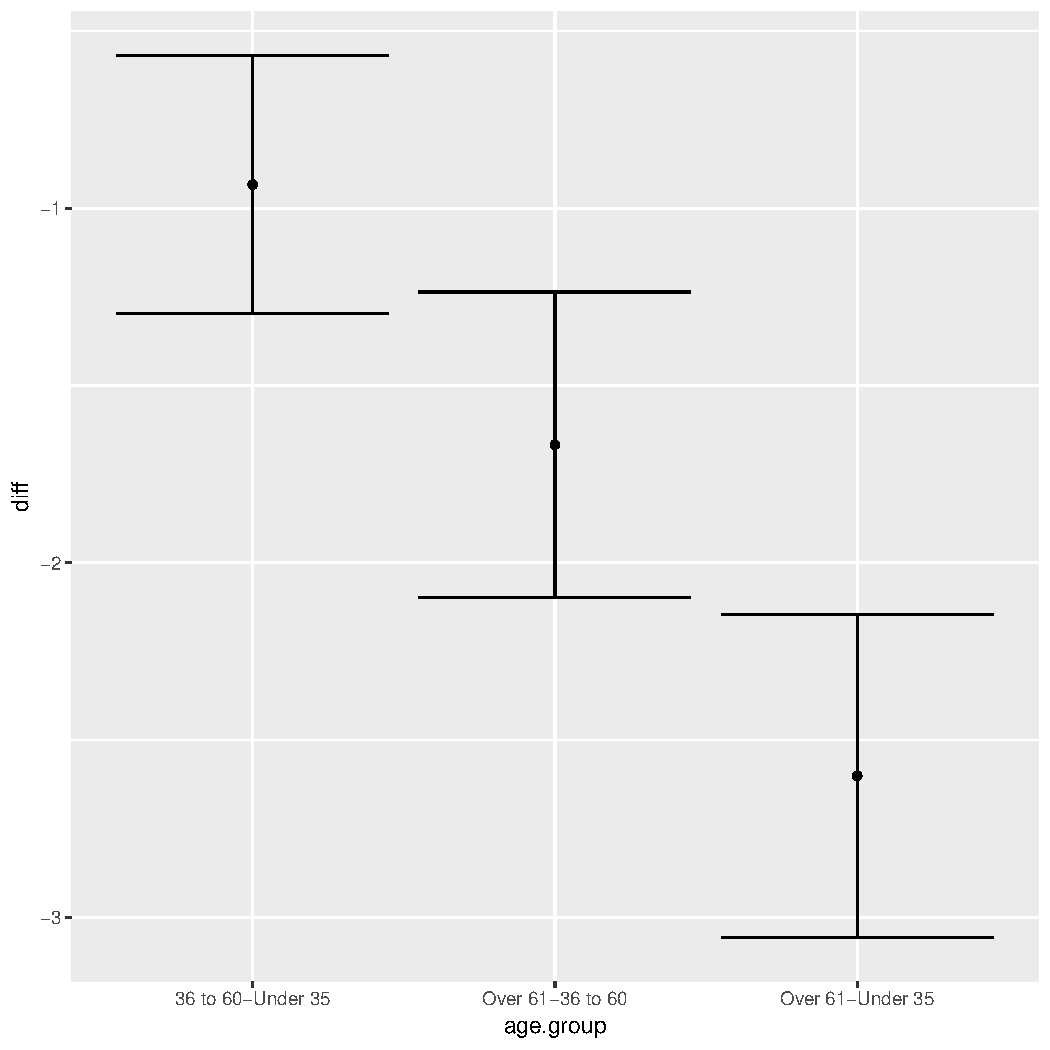
\includegraphics[width=0.6\linewidth]{figure/scat1-1} 

}



\end{knitrout}
\end{frame} 


\begin{frame}[fragile]
  \frametitle{Two-way ANOVA}
\begin{itemize} 
\item \texttt{tryaov} was fitted using one categorical explanatory variable (\texttt{age.group}). We therefore refer to its ANOVA table as \emph{one-way}.
\item If we fit a linear model using two categorical explanatory variables, we have a \emph{two-way} ANOVA.
\item Recall: All categorical variables should be converted into factors.
\begin{knitrout}
\definecolor{shadecolor}{rgb}{0.969, 0.969, 0.969}\color{fgcolor}\begin{kframe}
\begin{alltt}
\hlstd{issp.df}\hlopt{$}\hlstd{Gender} \hlkwb{<-} \hlkwd{factor}\hlstd{(issp.df}\hlopt{$}\hlstd{Gender)}
\hlstd{try2way} \hlkwb{<-} \hlkwd{with}\hlstd{(issp.df,}
                \hlkwd{aov}\hlstd{(total.lik}\hlopt{~}\hlstd{Gender}\hlopt{*}\hlstd{age.group))}
\end{alltt}
\end{kframe}
\end{knitrout}
\item \verb|Gender*age.group| is equivalent to \verb|Gender + age.group + Gender:age.group|.
\end{itemize}
\end{frame}

\begin{frame}[fragile]
  \frametitle{Two-way ANOVA}
\begin{knitrout}
\definecolor{shadecolor}{rgb}{0.969, 0.969, 0.969}\color{fgcolor}\begin{kframe}
\begin{alltt}
\hlkwd{summary}\hlstd{(try2way)}
\end{alltt}
\begin{verbatim}
                  Df Sum Sq Mean Sq F value   Pr(>F)    
Gender             1     98    97.7  22.200 2.82e-06 ***
age.group          2    774   386.8  87.905  < 2e-16 ***
Gender:age.group   2     15     7.3   1.654    0.192    
Residuals        947   4167     4.4                     
---
Signif. codes:  0 '***' 0.001 '**' 0.01 '*' 0.05 '.' 0.1 ' ' 1
94 observations deleted due to missingness
\end{verbatim}
\end{kframe}
\end{knitrout}
There is no two-way interaction between \texttt{Gender} and \texttt{age.group} ($p$-value = 0.19), i.e., the magnitude of the difference in mean total score between males and females is constant across all age groups, and vice versa.
\end{frame} 


\begin{frame}[fragile]
  \frametitle{Two-way ANOVA}
\begin{knitrout}
\definecolor{shadecolor}{rgb}{0.969, 0.969, 0.969}\color{fgcolor}\begin{kframe}
\begin{alltt}
\hlkwd{summary}\hlstd{(try2way)}
\end{alltt}
\begin{verbatim}
                  Df Sum Sq Mean Sq F value   Pr(>F)    
Gender             1     98    97.7  22.200 2.82e-06 ***
age.group          2    774   386.8  87.905  < 2e-16 ***
Gender:age.group   2     15     7.3   1.654    0.192    
Residuals        947   4167     4.4                     
---
Signif. codes:  0 '***' 0.001 '**' 0.01 '*' 0.05 '.' 0.1 ' ' 1
94 observations deleted due to missingness
\end{verbatim}
\end{kframe}
\end{knitrout}
We have extremly strong evidence that:
\begin{itemize}
\item the mean total score of {\em at least one} age group differs from the others, and
\item mean total score differs between males and females.
\end{itemize}
\end{frame} 

\begin{frame}[fragile]
  \frametitle{Estimated means}
\begin{knitrout}
\definecolor{shadecolor}{rgb}{0.969, 0.969, 0.969}\color{fgcolor}\begin{kframe}
\begin{alltt}
\hlkwd{model.tables}\hlstd{(try2way,} \hlstr{"means"}\hlstd{)}
\end{alltt}
\begin{verbatim}
Tables of means
Grand mean
         
12.43757 

 Gender 
    Female   Male
     12.71  12.06
rep 549.00 404.00

 age.group 
    Under 35 36 to 60 Over 61
       13.39    12.43   10.84
rep   319.00   445.00  189.00

 Gender:age.group 
        age.group
Gender   Under 35 36 to 60 Over 61
  Female  13.75    12.65    10.87 
  rep    184.00   271.00    94.00 
  Male    12.90    12.16    10.71 
  rep    135.00   174.00    95.00 
\end{verbatim}
\end{kframe}
\end{knitrout}
\end{frame} 


\begin{frame}[fragile]
  \frametitle{Post-hoc pairwise comparisons}
\begin{knitrout}
\definecolor{shadecolor}{rgb}{0.969, 0.969, 0.969}\color{fgcolor}\begin{kframe}
\begin{alltt}
\hlkwd{TukeyHSD}\hlstd{(try2way)}
\end{alltt}
\begin{verbatim}
  Tukey multiple comparisons of means
    95% family-wise confidence level

Fit: aov(formula = total.lik ~ Gender * age.group)

$Gender
                  diff        lwr        upr   p adj
Male-Female -0.6478476 -0.9176817 -0.3780135 2.8e-06

$age.group
                        diff       lwr        upr p adj
36 to 60-Under 35 -0.9533867 -1.314615 -0.5921584     0
Over 61-Under 35  -2.5488847 -3.000862 -2.0969079     0
Over 61-36 to 60  -1.5954980 -2.023006 -1.1679900     0

$`Gender:age.group`
                                      diff        lwr         upr
Male:Under 35-Female:Under 35   -0.8537037 -1.5324924 -0.17491498
Female:36 to 60-Female:Under 35 -1.1042435 -1.6764164 -0.53207073
Male:36 to 60-Female:Under 35   -1.5890805 -2.2224732 -0.95568776
Female:Over 61-Female:Under 35  -2.8776596 -3.6370492 -2.11827000
Male:Over 61-Female:Under 35    -3.0447368 -3.8014764 -2.28799724
Female:36 to 60-Male:Under 35   -0.2505398 -0.8815358  0.38045609
Male:36 to 60-Male:Under 35     -0.7353768 -1.4223705 -0.04838298
Female:Over 61-Male:Under 35    -2.0239559 -2.8285966 -1.21931516
Male:Over 61-Male:Under 35      -2.1910331 -2.9931734 -1.38889290
Male:36 to 60-Female:36 to 60   -0.4848369 -1.0667201  0.09704627
Female:Over 61-Female:36 to 60  -1.7734160 -2.4904058 -1.05642631
Male:Over 61-Female:36 to 60    -1.9404933 -2.6546757 -1.22631086
Female:Over 61-Male:36 to 60    -1.2885791 -2.0553117 -0.52184653
Male:Over 61-Male:36 to 60      -1.4556564 -2.2197645 -0.69154831
Male:Over 61-Female:Over 61     -0.1670773 -1.0384827  0.70432813
                                    p adj
Male:Under 35-Female:Under 35   0.0046497
Female:36 to 60-Female:Under 35 0.0000007
Male:36 to 60-Female:Under 35   0.0000000
Female:Over 61-Female:Under 35  0.0000000
Male:Over 61-Female:Under 35    0.0000000
Female:36 to 60-Male:Under 35   0.8672596
Male:36 to 60-Male:Under 35     0.0277926
Female:Over 61-Male:Under 35    0.0000000
Male:Over 61-Male:Under 35      0.0000000
Male:36 to 60-Female:36 to 60   0.1645240
Female:Over 61-Female:36 to 60  0.0000000
Male:Over 61-Female:36 to 60    0.0000000
Female:Over 61-Male:36 to 60    0.0000273
Male:Over 61-Male:36 to 60      0.0000010
Male:Over 61-Female:Over 61     0.9941396
\end{verbatim}
\end{kframe}
\end{knitrout}
\end{frame} 
 
%\begin{frame}[fragile]
%  \frametitle{Linear regression}
%<<fig.align ='center', out.width = '0.8\\textwidth', echo = F>>=
%with(issp.df, plot(Age, total.lik))
%@
%\end{frame} 

\begin{frame}[fragile]
  \frametitle{Test of independence}
\begin{knitrout}
\definecolor{shadecolor}{rgb}{0.969, 0.969, 0.969}\color{fgcolor}\begin{kframe}
\begin{alltt}
\hlstd{Q5.age.tab} \hlkwb{<-} \hlkwd{with}\hlstd{(issp.df,} \hlkwd{table}\hlstd{(Q5, age.group))}
\hlstd{Q5.age.tab}
\end{alltt}
\begin{verbatim}
                  age.group
Q5                 Under 35 36 to 60 Over 61
  be obedient            38       74      75
  think themselves      259      353     122
\end{verbatim}
\end{kframe}
\end{knitrout}
Do opinions on preparing children for life depend on age group? Statistically speaking, is \texttt{Q5} (the variable) and \texttt{age.group} independent of one another?
\end{frame} 

\begin{frame}[fragile]
  \frametitle{Pearson's Chi-squared test}
\begin{knitrout}
\definecolor{shadecolor}{rgb}{0.969, 0.969, 0.969}\color{fgcolor}\begin{kframe}
\begin{alltt}
\hlkwd{chisq.test}\hlstd{(Q5.age.tab)}
\end{alltt}
\begin{verbatim}

	Pearson's Chi-squared test

data:  Q5.age.tab
X-squared = 51.115, df = 2, p-value = 7.955e-12
\end{verbatim}
\end{kframe}
\end{knitrout}
\begin{itemize}
\item There is extremely strong evidence (\texttt{p}-value $<$ 0.0001) that \texttt{Q5} and \texttt{age.group} are not independent of one another.
\item Opinions on preparing children for life depend on the age group to which respondents belong.
\end{itemize}
\end{frame} 


\begin{frame}[fragile]
  \frametitle{Assumptions}
\begin{itemize}
\item Pearson's Chi-squared tests have certain assumptions. Beyond the scope of this course.
\item \texttt{chisq.test()} will give you a warning if these assumptions are not met.
\begin{knitrout}
\definecolor{shadecolor}{rgb}{0.969, 0.969, 0.969}\color{fgcolor}\begin{kframe}


{\ttfamily\noindent\color{warningcolor}{Warning in chisq.test(mytest): Chi-squared approximation may be incorrect}}\end{kframe}
\end{knitrout}
\item These assumptions are more likely to be wrong if the sample size is small.
\item If this happens, the alternative is to use Fisher's exact test.
\end{itemize}
\end{frame} 

\begin{frame}[fragile]
  \frametitle{Fisher's exact test}
Assume \texttt{Q5.age.tab} does not meet the underlying assumptions of Pearson's Chi-squared test.
\begin{knitrout}
\definecolor{shadecolor}{rgb}{0.969, 0.969, 0.969}\color{fgcolor}\begin{kframe}
\begin{alltt}
\hlkwd{fisher.test}\hlstd{(Q5.age.tab)}
\end{alltt}
\begin{verbatim}

	Fisher's Exact Test for Count Data

data:  Q5.age.tab
p-value = 6.93e-11
alternative hypothesis: two.sided
\end{verbatim}
\end{kframe}
\end{knitrout}
\end{frame} 

\begin{frame}[fragile]
  \frametitle{Summary}
  \begin{itemize}
  \item Student's $t$-test
  \item One-way ANOVA
  \item Two-way ANOVA
  \item Pearson’s Chi-squared test
  \item Fisher’s exact test
  \end{itemize}
\end{frame}

\end{document}     
